\documentclass[a4paper]{article}
\author{Буренин А.А}


% Packages
\usepackage{amsmath}
\usepackage[14pt]{extsizes}

\usepackage{fontspec}
\setromanfont{Times New Roman}

\usepackage[utf8]{inputenc}
\usepackage[russian]{babel}
\usepackage{multicol}
\usepackage[
a4paper,
left=30mm,
right=15mm,
top=20mm,
bottom=20mm,
nohead,
footskip=10mm
]{geometry}
\usepackage{graphicx}
\usepackage{textcomp}
\usepackage{tocloft}
\usepackage{titlesec}
\usepackage{ragged2e}
\usepackage{hyperref}
\usepackage{textcase}
\usepackage{sectsty}
\usepackage{sidecap}


\graphicspath{{./imgs/}}

% Подключает команду \mireatile
\newcommand{\mireatitle}[5]{{
    \clearpage
    \begin{center}
        
\includegraphics[width=30mm]{../static/logo}

        \footnotesize{МИНИСТЕРСТВО НАУКИ И ВЫСШЕГО ОБРАЗОВАНИЯ РОССИЙСКОЙ ФЕДЕРАЦИИ}

        \small
        Федеральное государственное бюджетное образовательное учреждение высшего образования

        \textbf{<<МИРЭА Российский технологический университет>>}

        \vspace{1.5em}

        \textbf{\large{РТУ МИРЭА}}
        \vspace{1.5em}

        \hline \hline

        \vspace{1.5em}

        \normalsize

        Институт информационных технологий

        Кафедра общей информатики

        \vspace{3em}

        \textbf{ОТЧЕТ}

        \textbf{ПО ПРАКТИЧЕСКОЙ РАБОТЕ № #1}

        \textbf{по дисциплине}

        <<ИНФОРМАТИКА>>


    \end{center}
    \vspace{6em}
    Выполнил студент группы #2 \hfill #3

    \vspace{1.7em}

    \flushleft{Принял \hfill #4}

    \textit{#5}

    \vspace{2em}


        \begin{tabular}{lrr}
            Практическая работа &
            <<\makebox[20pt][l]{\hrulefill}>>\makebox[80pt][r]{\hrulefill} 2022 г. &
            \makebox[30pt][k]{\hfill} \\

            выполнена \\

            <<Зачтено>> &
            <<\makebox[20pt][l]{\hrulefill}>>\makebox[80pt][r]{\hrulefill} 2022 г. &
            \makebox[30pt][k]{\hfill} \\

            \vspace*{\fill} % Заполняет пространство по вертикали
        \end{tabular}

    \begin{center}
        Москва, 2022
    \end{center}
    \thispagestyle{empty} % Убирает номер страницы
    \clearpage
}}


% Каким-то макаром делает загаловки в содержании
% написанными большими буквами
\makeatletter
\let\oldcontentsline\contentsline
\def\contentsline#1#2{%
	\expandafter\ifx\csname l@#1\endcsname\l@section
	\expandafter\@firstoftwo
	\else
	\expandafter\@secondoftwo
	\fi
	{%
		\oldcontentsline{#1}{\MakeTextUppercase{#2}}%
	}{%
		\oldcontentsline{#1}{#2}%
	}%
}
\makeatother


% Центрирует заголовок содержания
\renewcommand\cfttoctitlefont{\hfill\Large\mdseries}
\renewcommand\cftaftertoctitle{\hfill\mbox{}}

% Убирает полужирность у элементов содержания
\renewcommand\cftsecfont{\mdseries}

% Центрирует заголовки секций
\titleformat{\section}[block]{\large\bfseries\filcenter}{}{1em}{}
\sectionfont{\large\bfseries\centering}


\begin{document}
	
	% номер практики, номер группы, имя студента, имя преподавателя, должность преподавателя
	\mireatitle{5}{ИКБО-14-22}{Буренин А.А.}{Карпов Д.А.}{}
	
	\tableofcontents{}
	
	\clearpage
	
	
	\section{Постановка задачи}\label{sec:introduction}
	Логическая функция от четырех переменных задана в 16-теричной векторной форме. Восстановить таблицу истинности. По таблице истинности 
	реализовать в лабораторном комплексе логическую функцию на дешифраторах тремя способами:
	- используя дешифратор 4-16 и одну дополнительную схему «или»;
	- используя два дешифратора 3-8 и необходимую дополнительную логику;
	- используя пять дешифраторов 2-4 и одну дополнительную схему «или».
	Протестировать работу схем и убедиться в правильности их работы. 
	Подготовить отчет о проделанной работе и защитить ее.
	
	Логическая функция из персонального варианта:
	\[ F(a, b, c, d) = 6c6f_{16} \]
	
	
	\section{Проектирование и реализация}\label{sec:implementation}
	
	\subsection{Восстановление таблицы истинности}\label{subsec:table-recovering}
	Преобразовав 16-теричный вектор в двоичную СС, получаем восстановленную таблицу
	истинности для $ F $ (Таблица~\ref{tab:truth}).
	
	\begin{table}[h] 
		\begin{center}
			\begin{tabular}{ | c | c | c | c | c | }
				\hline
				$ a $ & $ b $ & $ c $ & $ d $ & $ F $ \\
				\hline
				0     & 0     & 0     & 0     & 0     \\
				\hline
				0     & 0     & 0     & 1     & 1     \\
				\hline
				0     & 0     & 1     & 0     & 0     \\
				\hline
				0     & 0     & 1     & 1     & 1     \\
				\hline
				0     & 1     & 0     & 0     & 1     \\
				\hline
				0     & 1     & 0     & 1     & 0     \\
				\hline
				0     & 1     & 1     & 0     & 1     \\
				\hline
				0     & 1     & 1     & 1     & 0     \\
				\hline
				1     & 0     & 0     & 0     & 0     \\
				\hline
				1     & 0     & 0     & 1     & 1     \\
				\hline
				1     & 0     & 1     & 0     & 1     \\
				\hline
				1     & 0     & 1     & 1     & 1     \\
				\hline
				1     & 1     & 0     & 0     & 0     \\
				\hline
				1     & 1     & 0     & 1     & 1     \\
				\hline
				1     & 1     & 1     & 0     & 1     \\
				\hline
				1     & 1     & 1     & 1     & 1     \\
				\hline
			\end{tabular}
		\end{center}
		\caption{Таблица истинности}
		\label{tab:truth}
	\end{table}
	
	\subsection{Реализация логической функции на дешифраторе 4-16}
	Реализуем функцию, используя дешифратор 4-16 и дополнительной схемы “или”. Для этого нам необходимо разместить его в лабораторном комплексе и выставить необходимые нам параметры. Так как количество адресных входов дешифратора равно количеству аргументов функции, мы просто подаем наши переменные на вход дешифратора через объединяющую шину. При этом значение переменной $ a $ подается на старший адресный вход, а $ d $ – на младший. Далее нужно выбрать те выходы дешифратора, номера которых совпадают с номерами наборов значений аргументов, при которых функция равна единице. Объединив эти выходы дизъюнкцией, получаем требуемую реализацию (Рисунок \ref{img:decoder-4-16}).
	
	\begin{figure}[h]
		\centering
		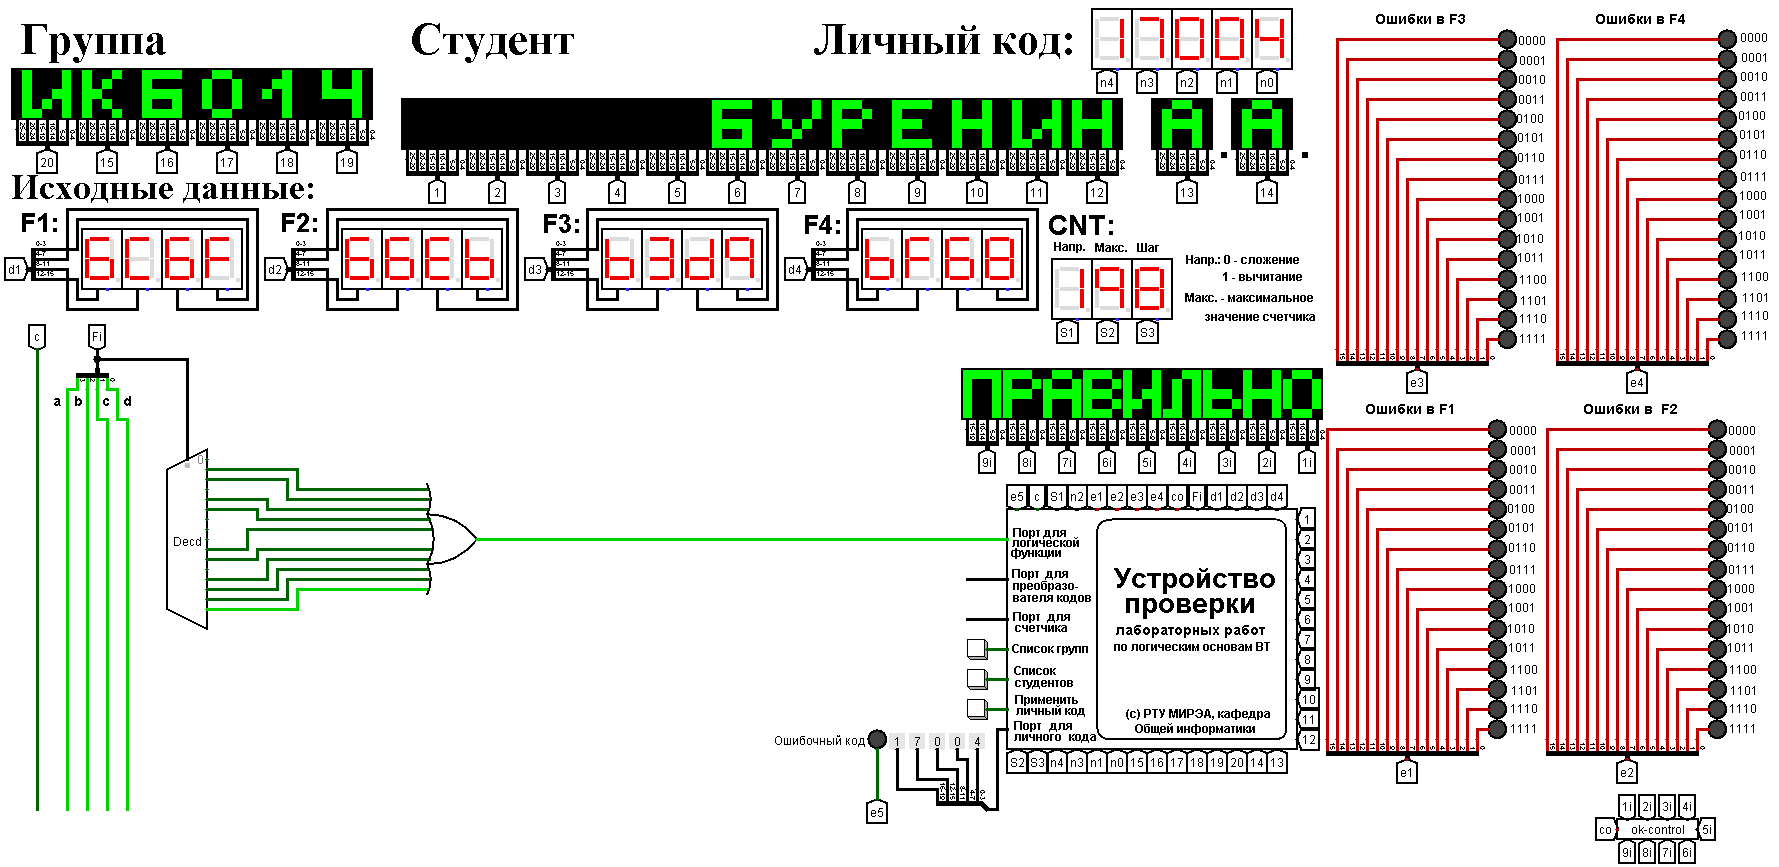
\includegraphics[width=0.8\textwidth]{4-16.png}
		\caption{\centering Реализация логической функции с помощью дешифратора 4-16.}\label{img:decoder-4-16}

	\end{figure}
	
	\subsection{Реализация логической функции на дешифраторе 3-8}
	Реализуем функцию, используя два дешифратора 3-8 и необходимую дополнительную логику. Для этого нам необходимо подать значение переменной $ а $ на их разрешающие входы, причем на первый дешифратор оно будет передаваться через инверсию. Это связано с тем, что в первой половине таблицы истинности значение $ а $ равно 0, а во второй – 1, что и позволяет разделить изначальный дешифратор 4-16 на два дешифратора 3-8, один из которых включается в зависимости от значения переменной $ а $. 
	
	Далее нужно подать значения оставшихся трех переменных на адресные входы дешифратора. Значение переменной $ b $ подается на старший вход, а значение переменной $ d $ – на младший. В процессе работы на выходах всех дешифраторов будут последовательно возникать единичные значения в соответствии с поступающей на адресные входы комбинацией значений переменных. У первого дешифратора выберем только те выходы, номера которых соответствуют номерам комбинаций переменных, в которых функция равна единице в первой половине таблицы истинности. Аналогичную операцию проделываем со вторым дешифратором для второй половиной таблицы. После объединения выходов дизъюнкцией получаем требуемую реализацию (Рисунок \ref{img:decoder-3-8}).
	
	\begin{figure}[h]
		\centering
		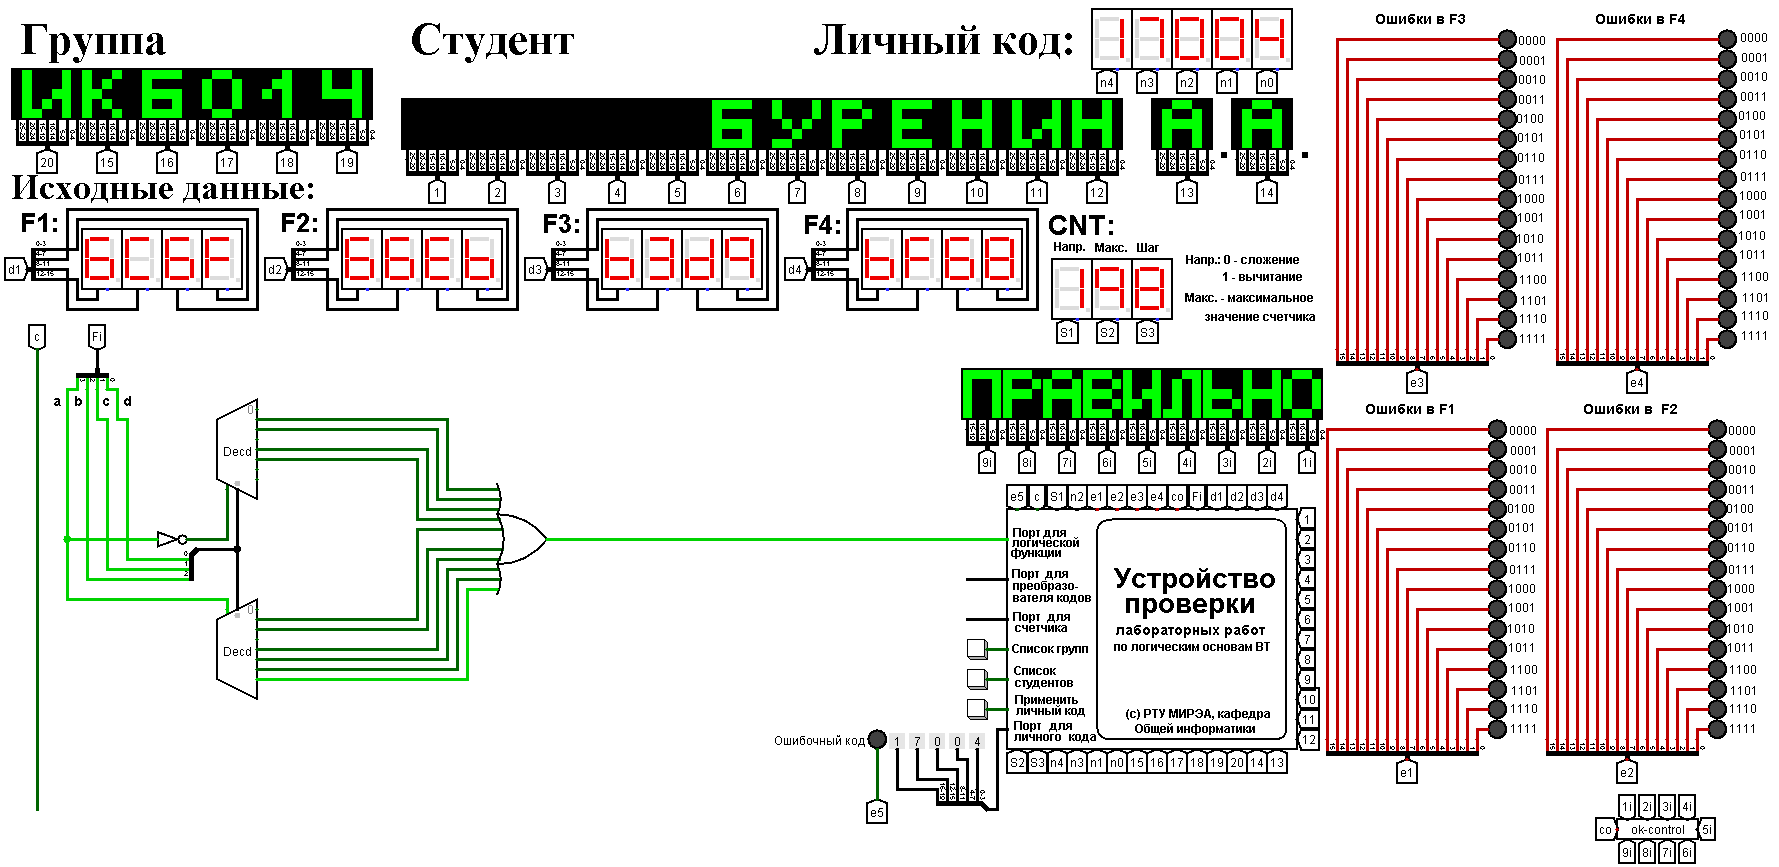
\includegraphics[width=0.8\textwidth]{3-8.png}
		
		\caption{\centering Реализация логической функции с помощью двух дешифраторов 3-8.}
		\label{img:decoder-3-8}
	\end{figure}
	
	\subsection{Реализация логической функции на дешифраторах 2-4}
	
	Теперь реализуем логическую функцию, используя дешифраторы 2-4 и дополнительную логику. Так как количество адресных входов таких дешифраторов в два раза меньше количества аргументов функции, то нам потребуется 4 дешифратора, которые будут называться операционными и один дешифратор, который будет ими управлять. Он будет называться управляющим. Всего будет использовано 5 дешифраторов и 2-4 и одна объединяющая дизъюнкция. При такой реализации значения двух старших переменных будут подаваться на адресные входы управляющего дешифратора, который будет включать один из четырех операционных дешифраторов в соответствии с комбинацией значений $ a $ и $ b $. Всего таких комбинаций четыре: 00, 01, 10 и 11. Выходы управляющего дешифратора подключаются к разрешающим входам операционных. Когда значения старших переменных равны 0, на нулевом выходе управляющего дешифратора образуется единица, которая подается на разрешающий вход первого операционного дешифратора. Аналогично с остальными значениями $ a $ и $ b $. 
	
	Теперь каждый из операционных дешифраторов отвечает за свою двоичную тетраду в исходной векторной записи логической функции. Выберем у каждого операционного дешифратора выходы, где у двоичной тетрады стоят единицы. Объединив эти выходы через дизъюнкцию получаем требуемую реализацию (Рисунок \ref{img:decoder-2-4}).
	
	\begin{figure}[h]
		\centering
		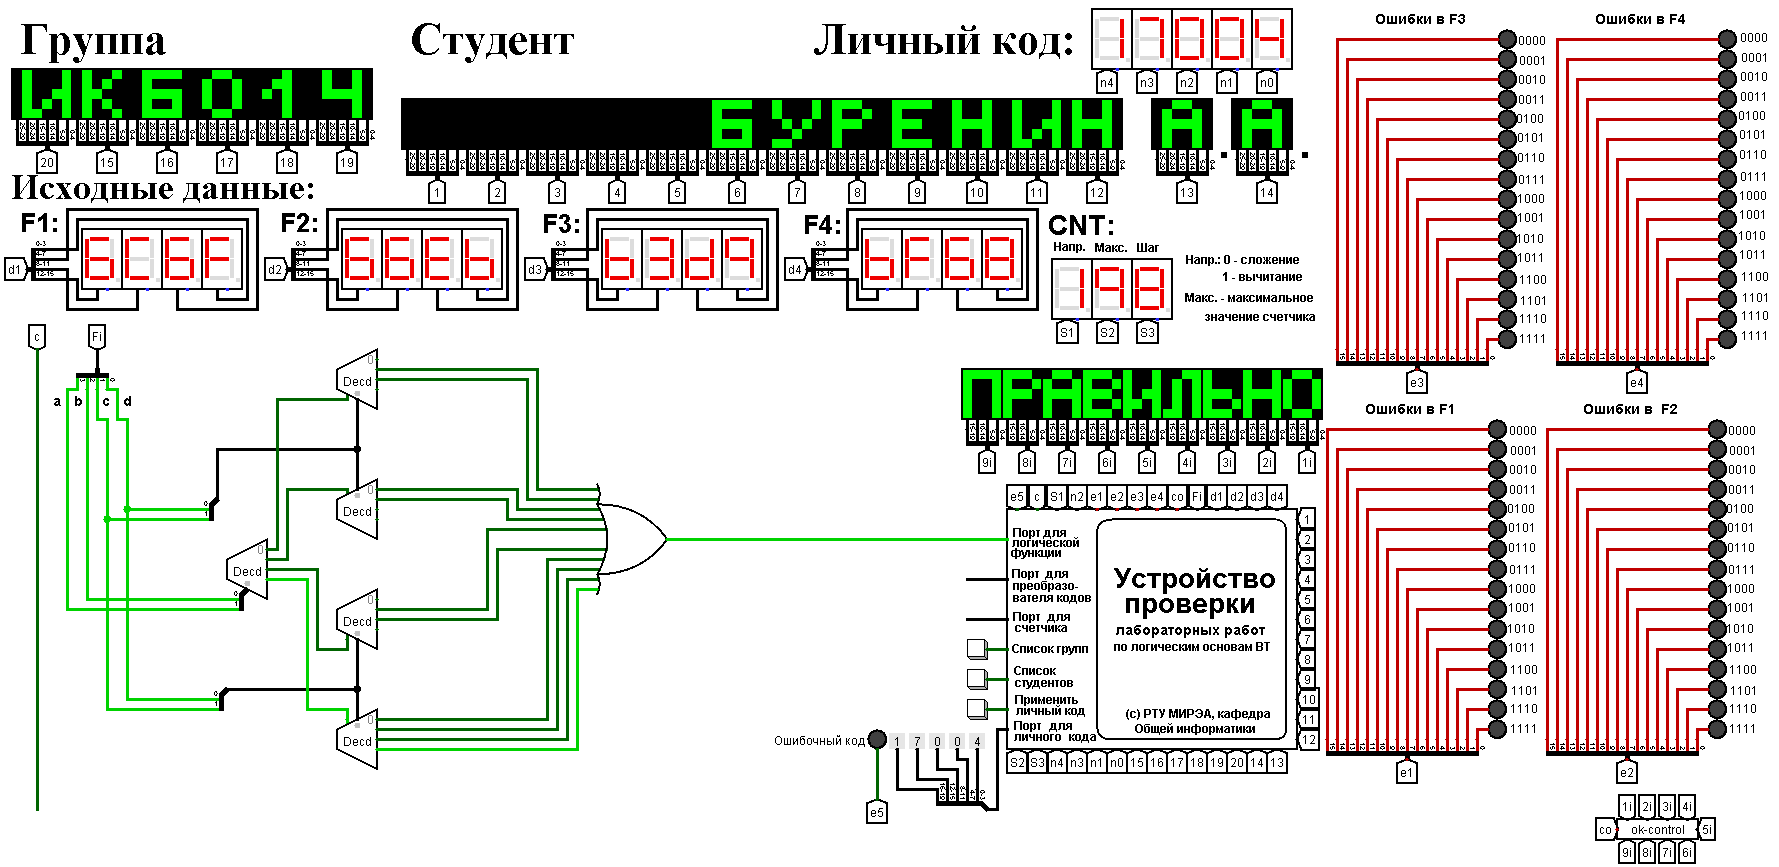
\includegraphics[width=0.8\textwidth]{2-4.png}
		
		\caption{\centering Реализация логической функции с помощью дешифраторов 2-4.}
		\label{img:decoder-2-4}
	\end{figure}
	
	
	\section{Выводы}\label{sec:conclusion}
	В ходе работы была восстановлена таблица истинности для данной логической функции, заданной в 16-теричной векторной форме (Таблица \ref{tab:truth}). По таблице истинности была реализована в лабораторном комплексе логическая функция на дешифраторах тремя способами:
	\begin{enumerate}
	\item используя дешифратор 4-16 и одну дополнительную схему «или» (Рисунок \ref{img:decoder-4-16});
	\item используя два дешифратора 3-8 и необходимую дополнительную логику (Рисунок \ref{img:decoder-3-8});
	\item используя пять дешифраторов 2-4 и одну дополнительную схему «или» (Рисунок \ref{img:decoder-2-4}).
	\end{enumerate}
	
	
	
	
	\section{Информационные источники}\label{sec:sources}
	\begin{enumerate}
		\item Информатика: Методические указания по выполнению практических 
		работ / С.С. Смирнов, Д.А. Карпов - М., МИРЭА - Российский технологический университет, 2020.–102 с.
		\item Лекционный материал / С.С. Смирнов.
	\end{enumerate}
	
\end{document}
